\documentclass{article}

%%% Fill details here (in the second brackets)
\newcommand{\name}{Hao Sun}     % Your name (First Last)
\newcommand{\wustlkey}{sun.hao}             % Your WUSTL Key
%%%



%%%%%%%%%%%%%%%%%%%%%% Formatting Stuff %%%%%%%%%%%%%%%%%%%%%%%%%%%
\usepackage{times}
\usepackage[T1]{fontenc}

\setlength{\parskip}{1em}\setlength{\parindent}{0pt}
\linespread{1.25}
\usepackage[margin=0.7in,top=1in]{geometry}\usepackage{fancyhdr}
\pagestyle{fancy}\lhead{\bf \name}\rhead{\bf \wustlkey}\cfoot{\thepage}
\newcommand{\info}{\clearpage \subsection*{Information}}

\newcommand{\solution}[1]{\clearpage \subsection*{Solution #1}}  % define a new command \solution without index number
\newcommand{\spart}[1]{\paragraph{(#1)}} 
%%%%%%%%%%%%%%%%%%%%%%%%%%%%%%%%%%%%%%%%%%%%%%%%%%%%%%%%%%%%%%%%%%%


%%% Add any more packages if you want to
\usepackage{amsmath,graphicx}


\begin{document}
%%%%% Main Body goes here

% Begin solution to every problem like this.
\solution{1}

\spart{a} 
Finding cluster centers:
\begin{figure*}[h!]
  \centering
	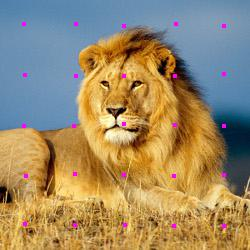
\includegraphics[height=15em]{code/outputs/prob1a_25_centers.jpg}
	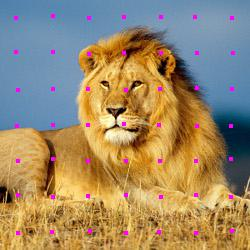
\includegraphics[height=15em]{code/outputs/prob1a_49_centers.jpg}
	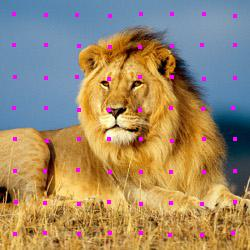
\includegraphics[height=15em]{code/outputs/prob1a_64_centers.jpg}
	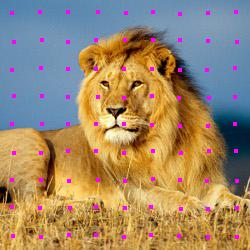
\includegraphics[height=15em]{code/outputs/prob1a_81_centers.jpg}
	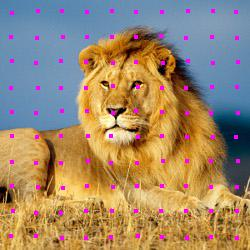
\includegraphics[height=15em]{code/outputs/prob1a_100_centers.jpg}
	\caption{Cluster centers 25, 49, 64, 81, 100}
\end{figure*}

\newpage
\spart{b} 
Finding superpixels with 25, 49, 64, 81, 100
\begin{figure*}[h!]
  \centering
	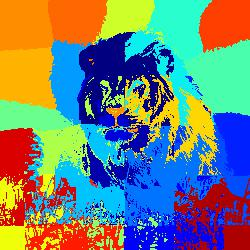
\includegraphics[height=15em]{code/outputs/prob1b_spatial_weight_0.7/prob1b_25.jpg}
	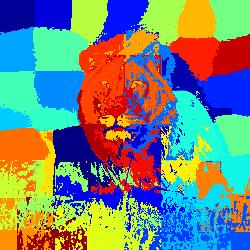
\includegraphics[height=15em]{code/outputs/prob1b_spatial_weight_0.7/prob1b_49.jpg}
	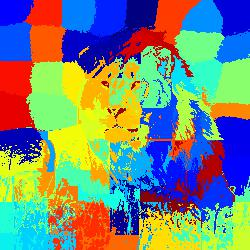
\includegraphics[height=15em]{code/outputs/prob1b_spatial_weight_0.7/prob1b_64.jpg}
	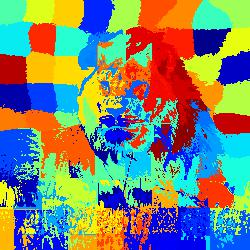
\includegraphics[height=15em]{code/outputs/prob1b_spatial_weight_0.7/prob1b_81.jpg}
	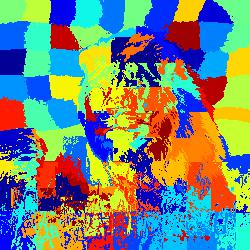
\includegraphics[height=15em]{code/outputs/prob1b_spatial_weight_0.7/prob1b_100.jpg}
	\caption{Superpixels 25, 49, 64, 81, 100 with spatial weight 0.7}
\end{figure*}

The spatial weight I choose is 0.7. If the spatial weight is approaching 1.0, the superpixel will become more like a square; if the spatial weight is approaching 0.0, the superpixel will become more irregular, because under this circumstance, the cluster is more determined by the intensities of R, G and B. As shown in the following figures.

\begin{figure*}[h!]
  \centering
	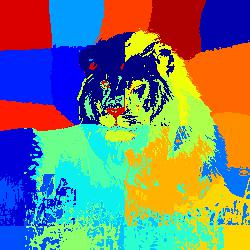
\includegraphics[height=15em]{code/outputs/prob1b_spatial_weight_1.0/prob1b_25.jpg}
	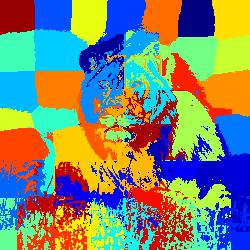
\includegraphics[height=15em]{code/outputs/prob1b_spatial_weight_1.0/prob1b_49.jpg}
	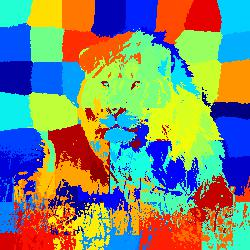
\includegraphics[height=15em]{code/outputs/prob1b_spatial_weight_1.0/prob1b_64.jpg}
	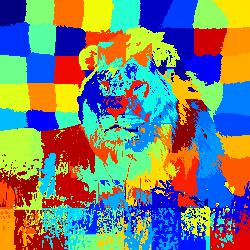
\includegraphics[height=15em]{code/outputs/prob1b_spatial_weight_1.0/prob1b_81.jpg}
	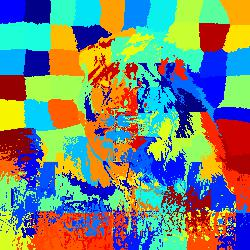
\includegraphics[height=15em]{code/outputs/prob1b_spatial_weight_1.0/prob1b_100.jpg}
	\caption{Superpixels 25, 49, 64, 81, 100 with spatial weight 1.0}
\end{figure*}

\begin{figure*}[h!]
  \centering
	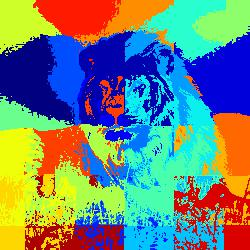
\includegraphics[height=15em]{code/outputs/prob1b_spatial_weight_0.3/prob1b_25.jpg}
	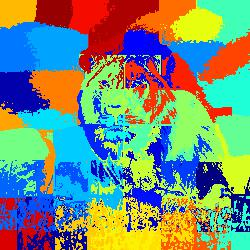
\includegraphics[height=15em]{code/outputs/prob1b_spatial_weight_0.3/prob1b_49.jpg}
	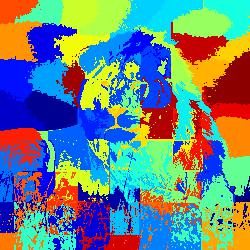
\includegraphics[height=15em]{code/outputs/prob1b_spatial_weight_0.3/prob1b_64.jpg}
	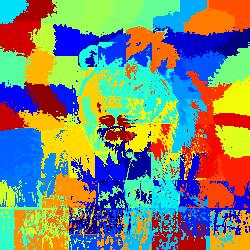
\includegraphics[height=15em]{code/outputs/prob1b_spatial_weight_0.3/prob1b_81.jpg}
	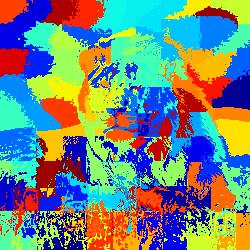
\includegraphics[height=15em]{code/outputs/prob1b_spatial_weight_0.3/prob1b_100.jpg}
	\caption{Superpixels 25, 49, 64, 81, 100 with spatial weight 0.3}
\end{figure*}

\solution{2}
\spart{a}
When I tried BSZ=50, lr = 0.075 and nHidden = 1024, I got the best performance, the training accuracy reached $100\%$ and Val accuracy reached $97.70\%$ after 50 epoches. As shown in the following screenshot.
\begin{figure*}[h!]
  \centering
	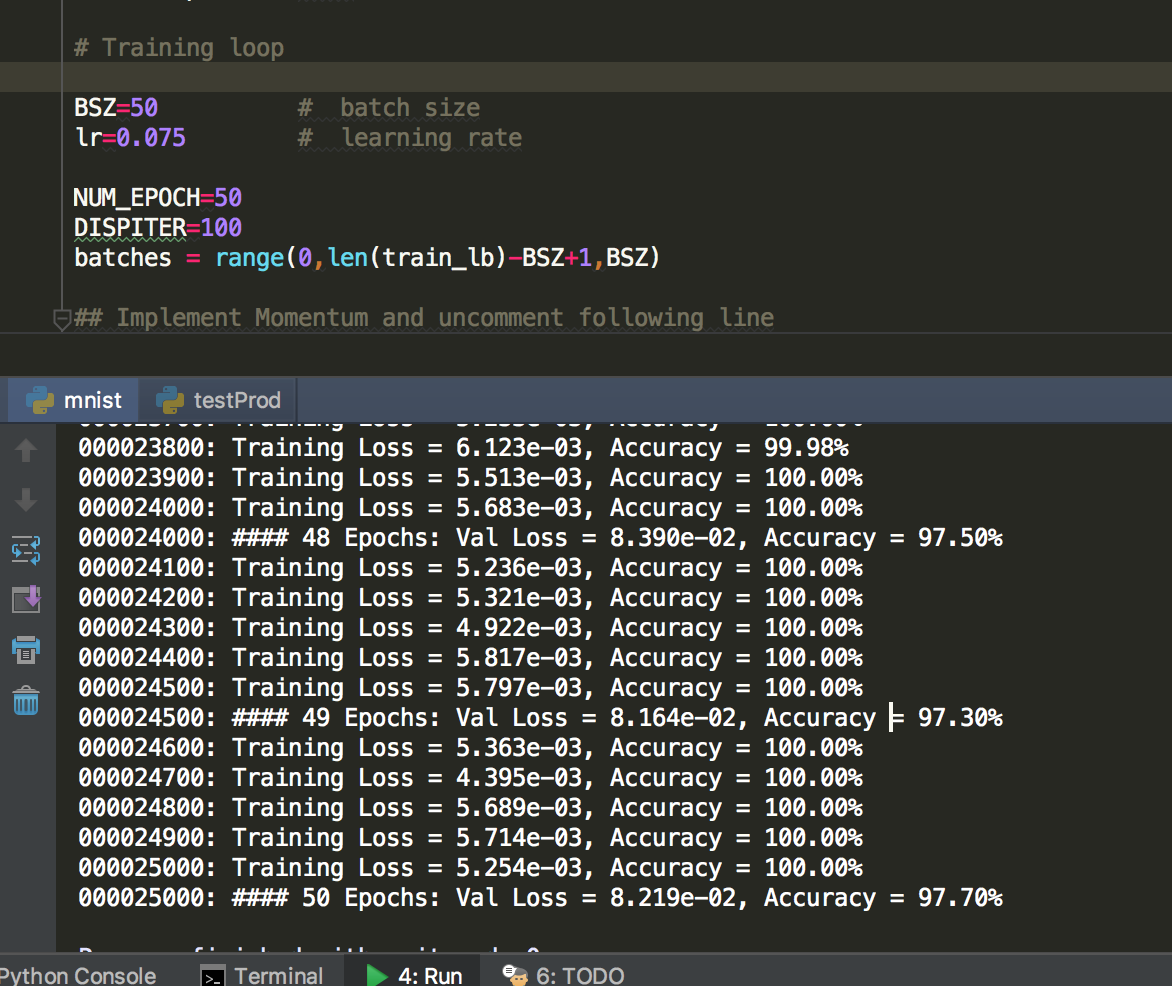
\includegraphics[height=25em]{screenshots/prob2(a)50_0075_1024.png}
	\caption{Training under BSZ=50, lr = 0.075 and nHidden = 1024}
\end{figure*}
\begin{figure*}[h!]
  \centering
	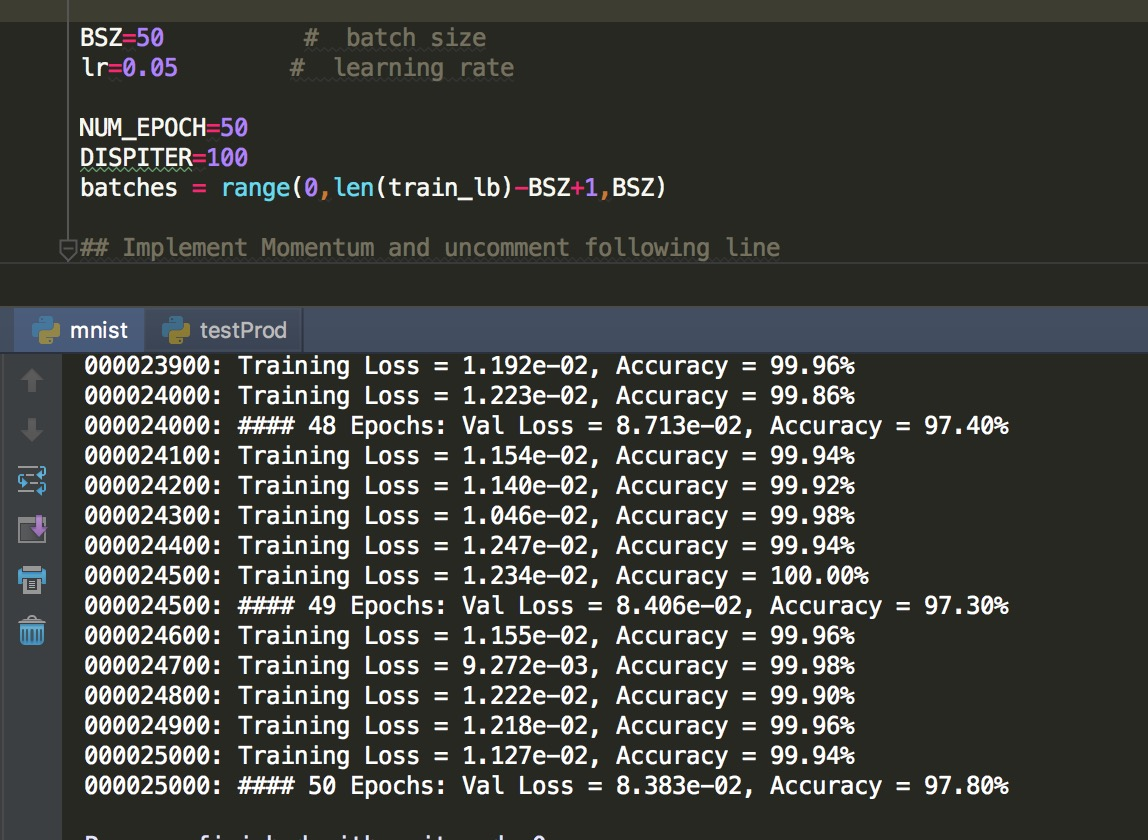
\includegraphics[height=25em]{screenshots/prob2(a)50-005-1024.png}
	\caption{Training under BSZ=50, lr = 0.05 and nHidden = 1024}
\end{figure*}
\begin{figure*}[h!]
  \centering
	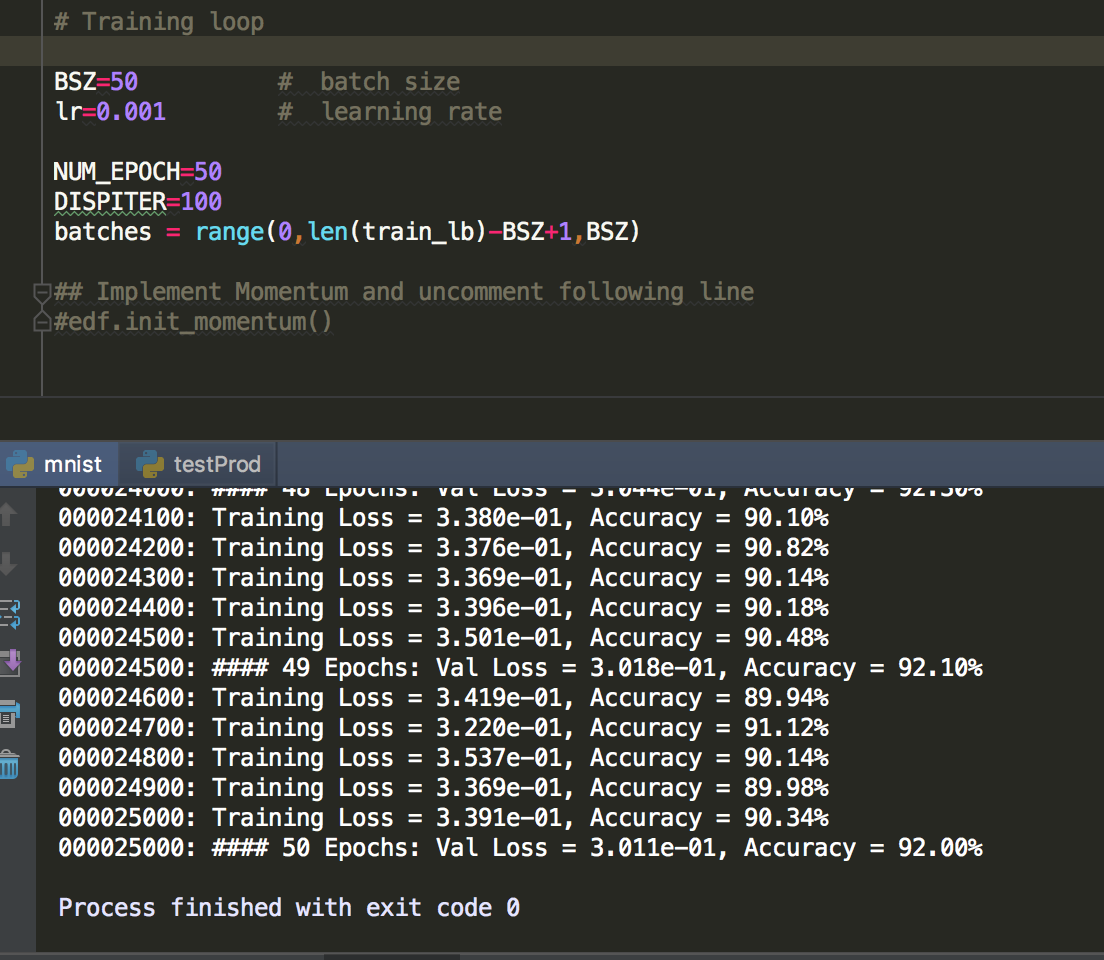
\includegraphics[height=25em]{screenshots/prob2(a)50-0001-1024.png}
	\caption{Training under BSZ=50, lr = 0.001 and nHidden = 1024}
\end{figure*}
\begin{figure*}[h!]
  \centering
	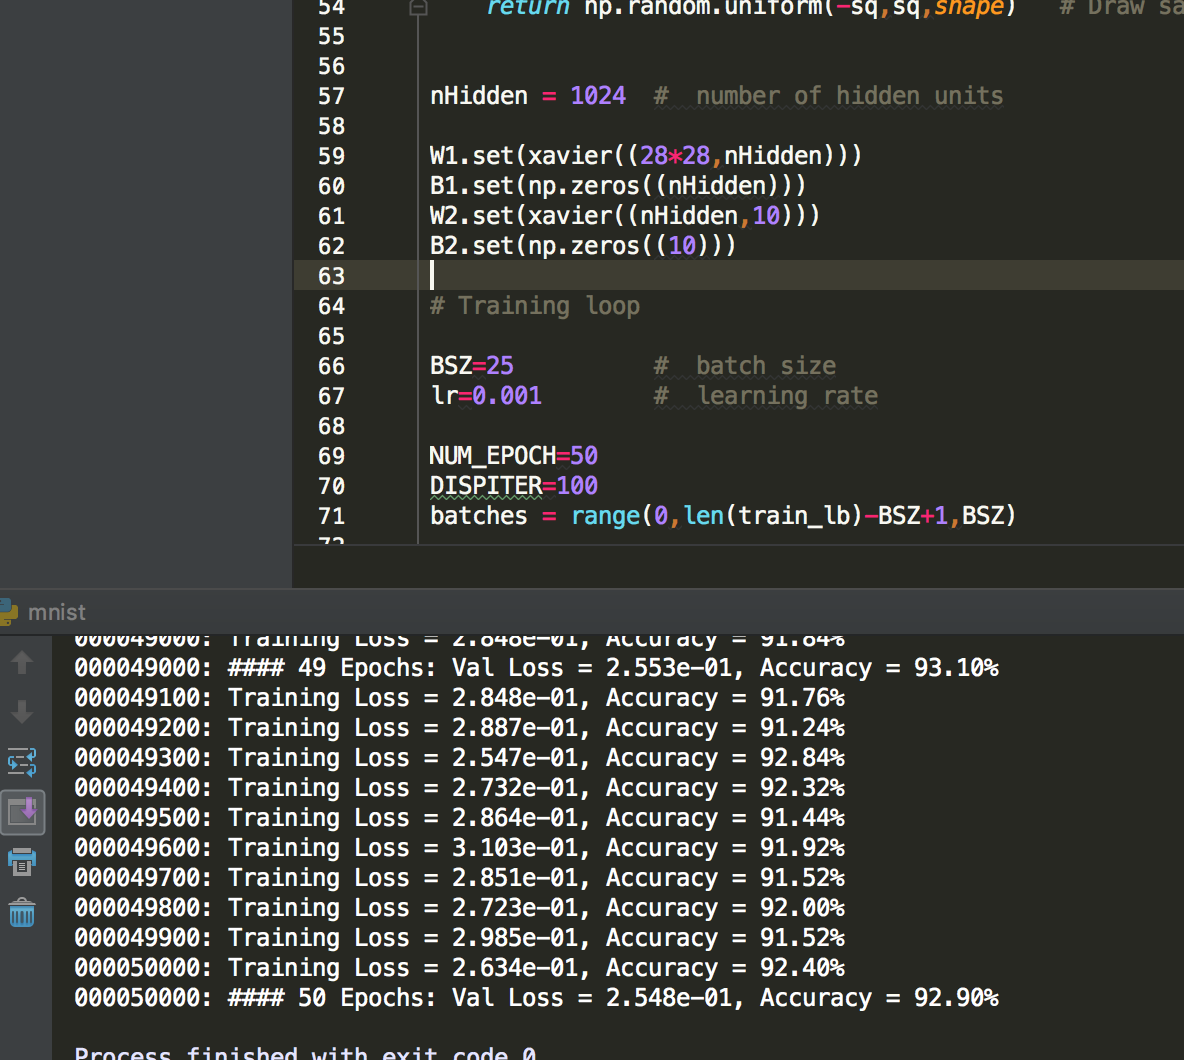
\includegraphics[height=25em]{screenshots/prob2(a)25-0001-1024.png}
	\caption{Training under BSZ=25, lr = 0.001 and nHidden = 1024}
\end{figure*}

\newpage
After several times of experiments, I verified the relationship between batch size and learning rate, that is smaller learning rate with smaller batch size, bigger learning rate with bigger batch size. Because with smaller batch size, after one batch training, program is less sure about the gradient, so "step size" (learning rate) should also be smaller. The number of hidden units represents the num of input features, the relation between classifier performance and number of hidden units is: less hidden units -> running faster -> lower accuracy; more hidden units -> running slower -> higher accuracy.

The limit of the uniform distribution being chosen in the way as function $xavier$ does is because: we have to make sure that weights are not too small and not too big to propagate accurately the signals.
\spart{b}
Implementing batched stochastic gradient descent with using momentum makes classifier training run faster and have higher accuracy. As showing in the following figures:

\begin{figure*}[h!]
  \centering
	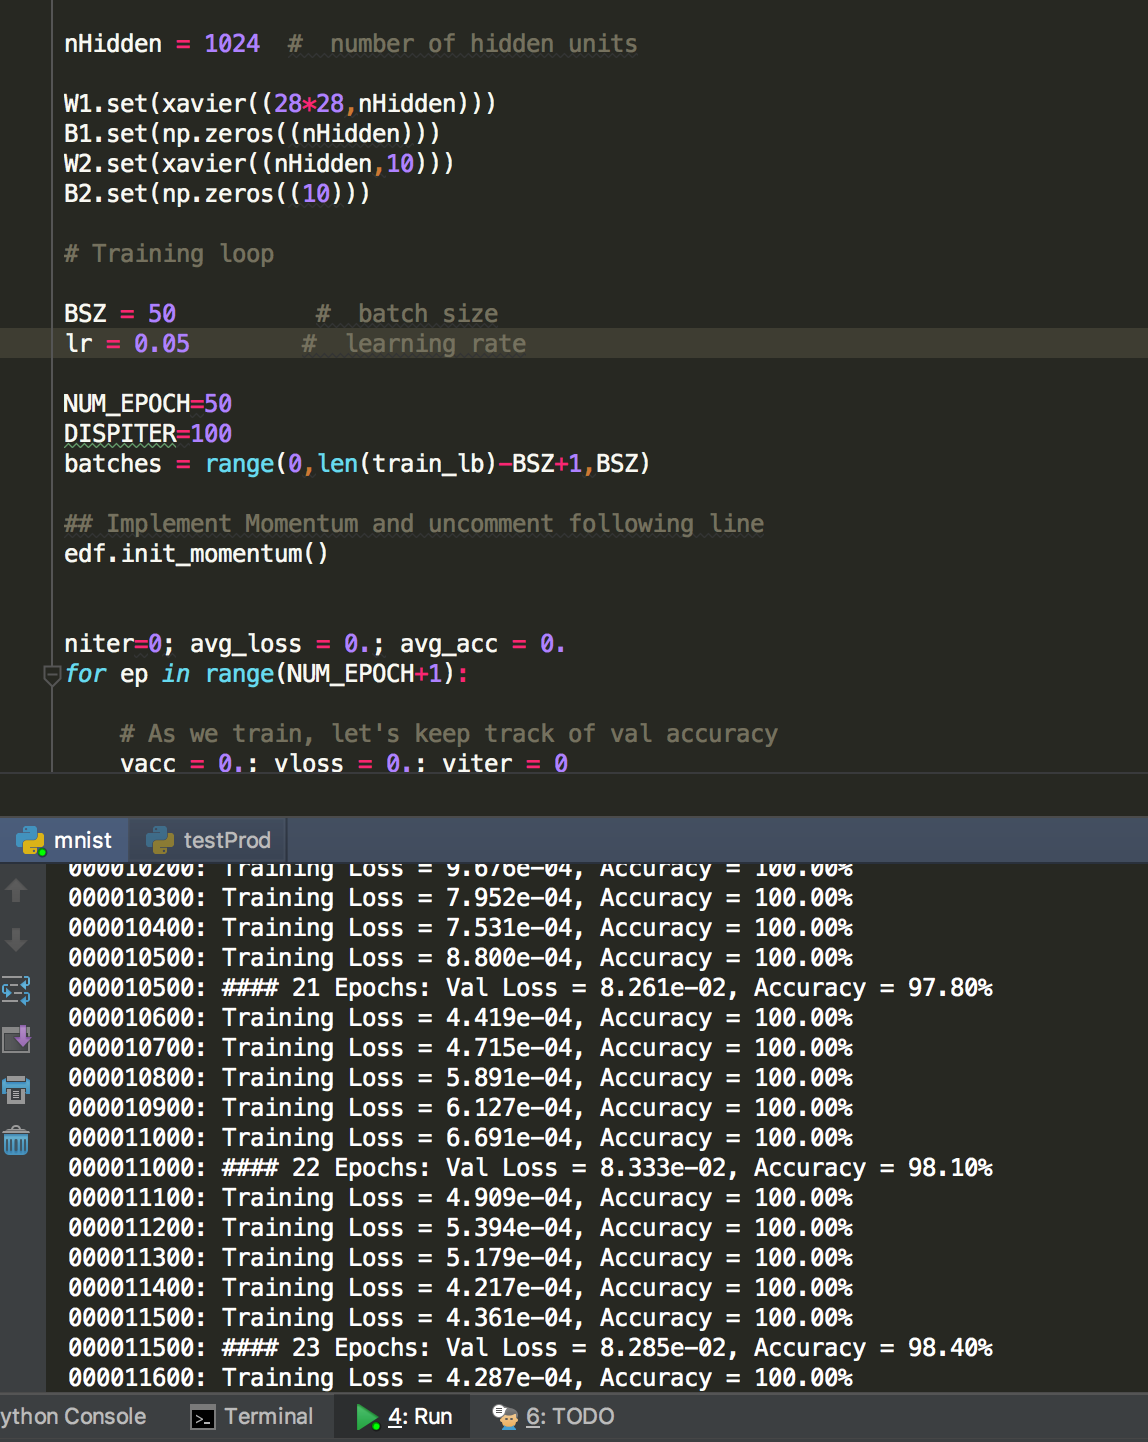
\includegraphics[height=40em]{screenshots/prob2(b)50-005-1024-1.png}
	\caption{Processing: Training with momentum under BSZ=50, lr = 0.05 and nHidden = 1024}
\end{figure*}

\begin{figure*}[h!]
  \centering
	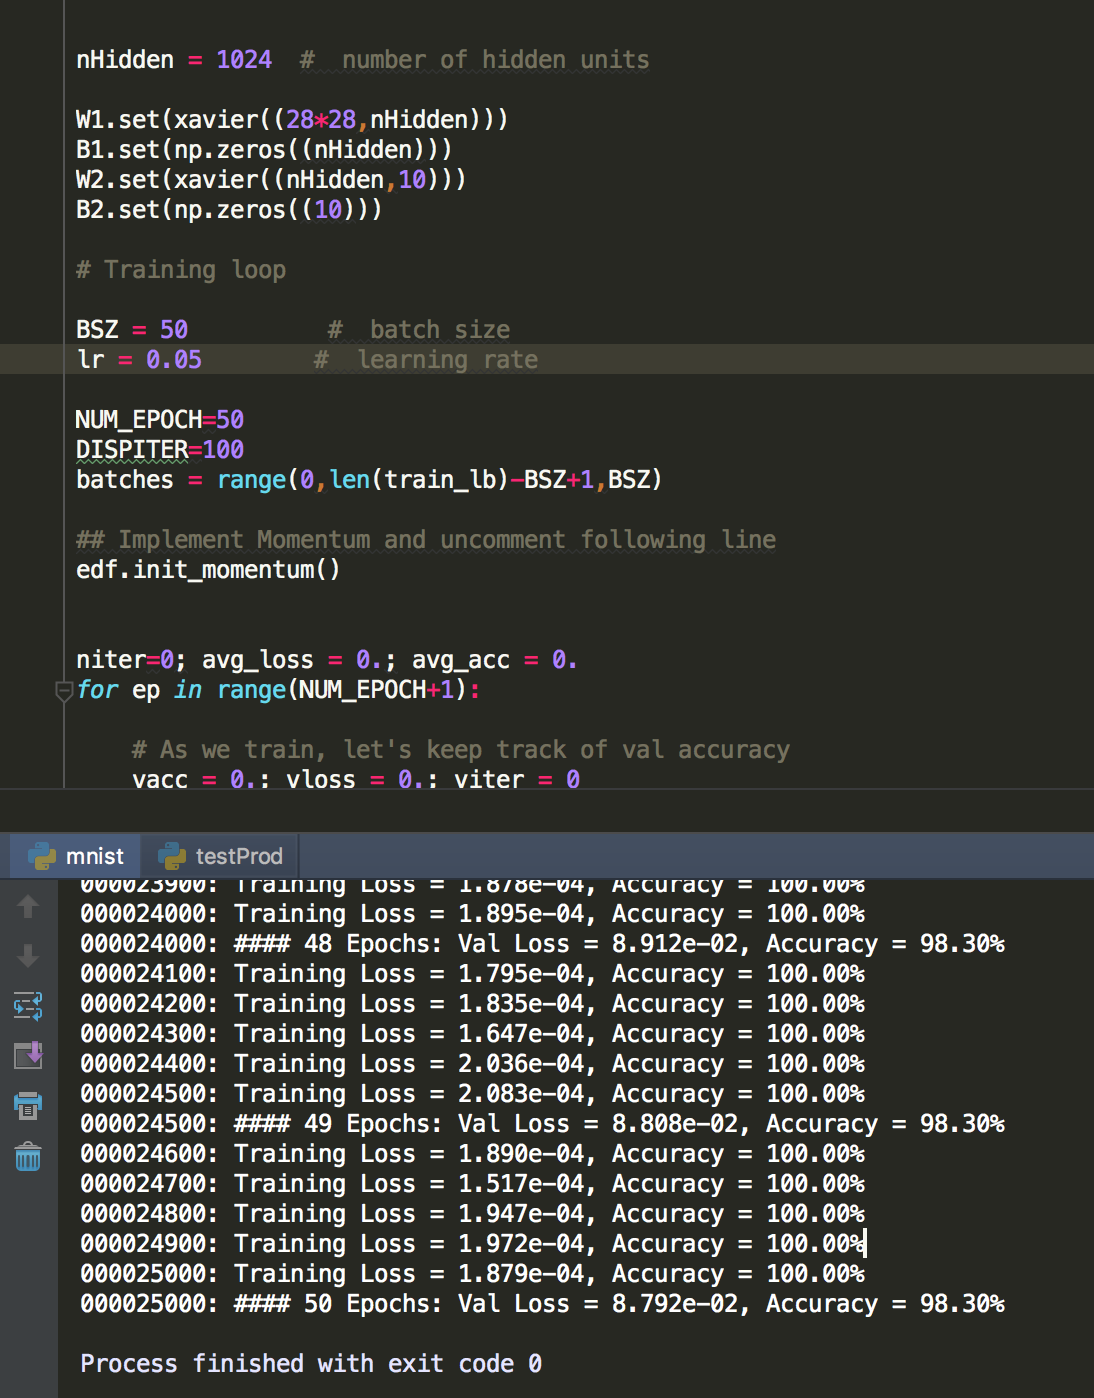
\includegraphics[height=40em]{screenshots/prob2(b)50-005-1024-3.png}
	\caption{Finished: Training with momentum under BSZ=50, lr = 0.05 and nHidden = 1024}
\end{figure*}

\solution{3}
The training results with one convolution layer:
\begin{figure*}[h!]
  \centering
	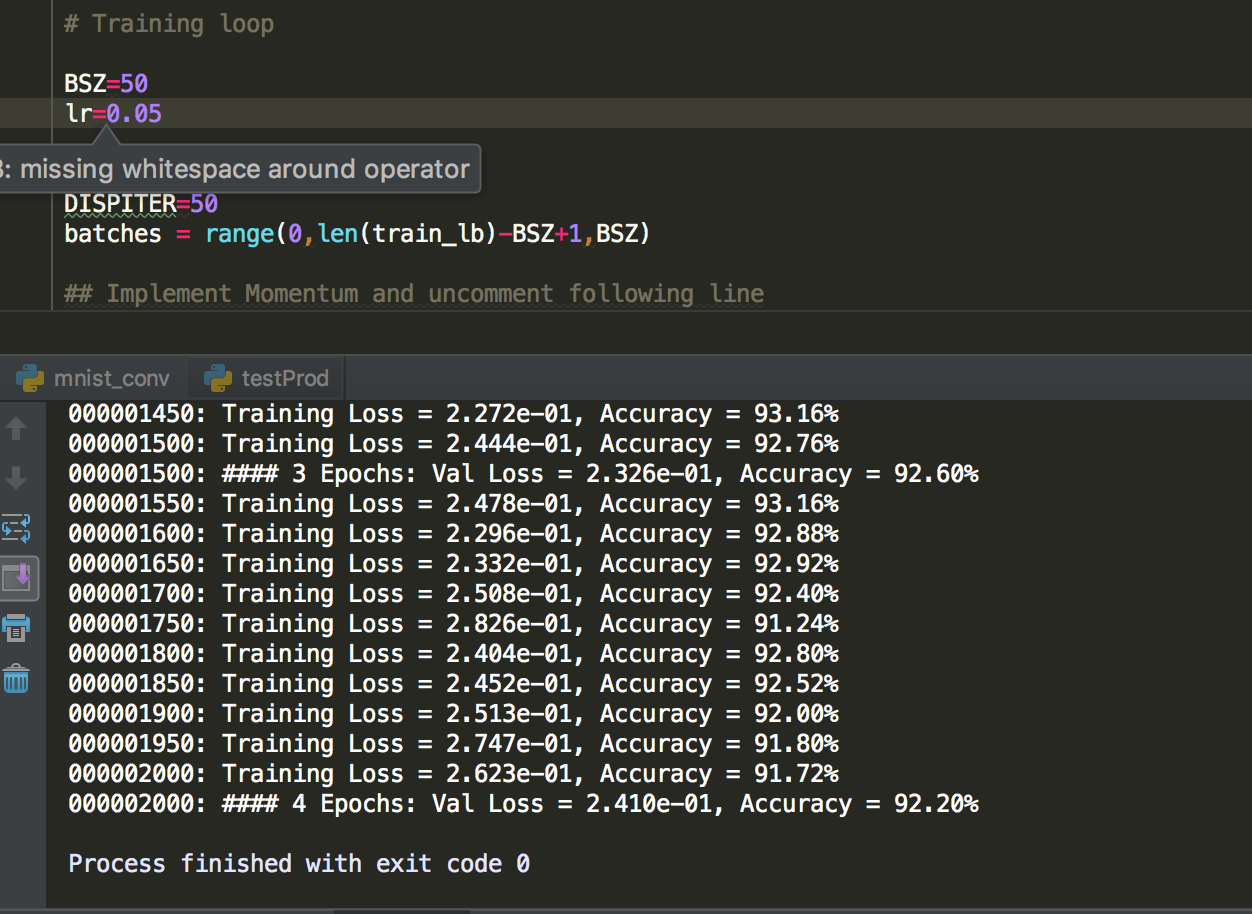
\includegraphics[height=20em]{screenshots/prob350-005-64.png}
	\caption{Processing: Training with momentum under BSZ=50, lr = 0.05 and C1 = 64}
\end{figure*}
%\newpage
\newline
The training results with two convolution layers:
\begin{figure*}[h!]
  \centering
	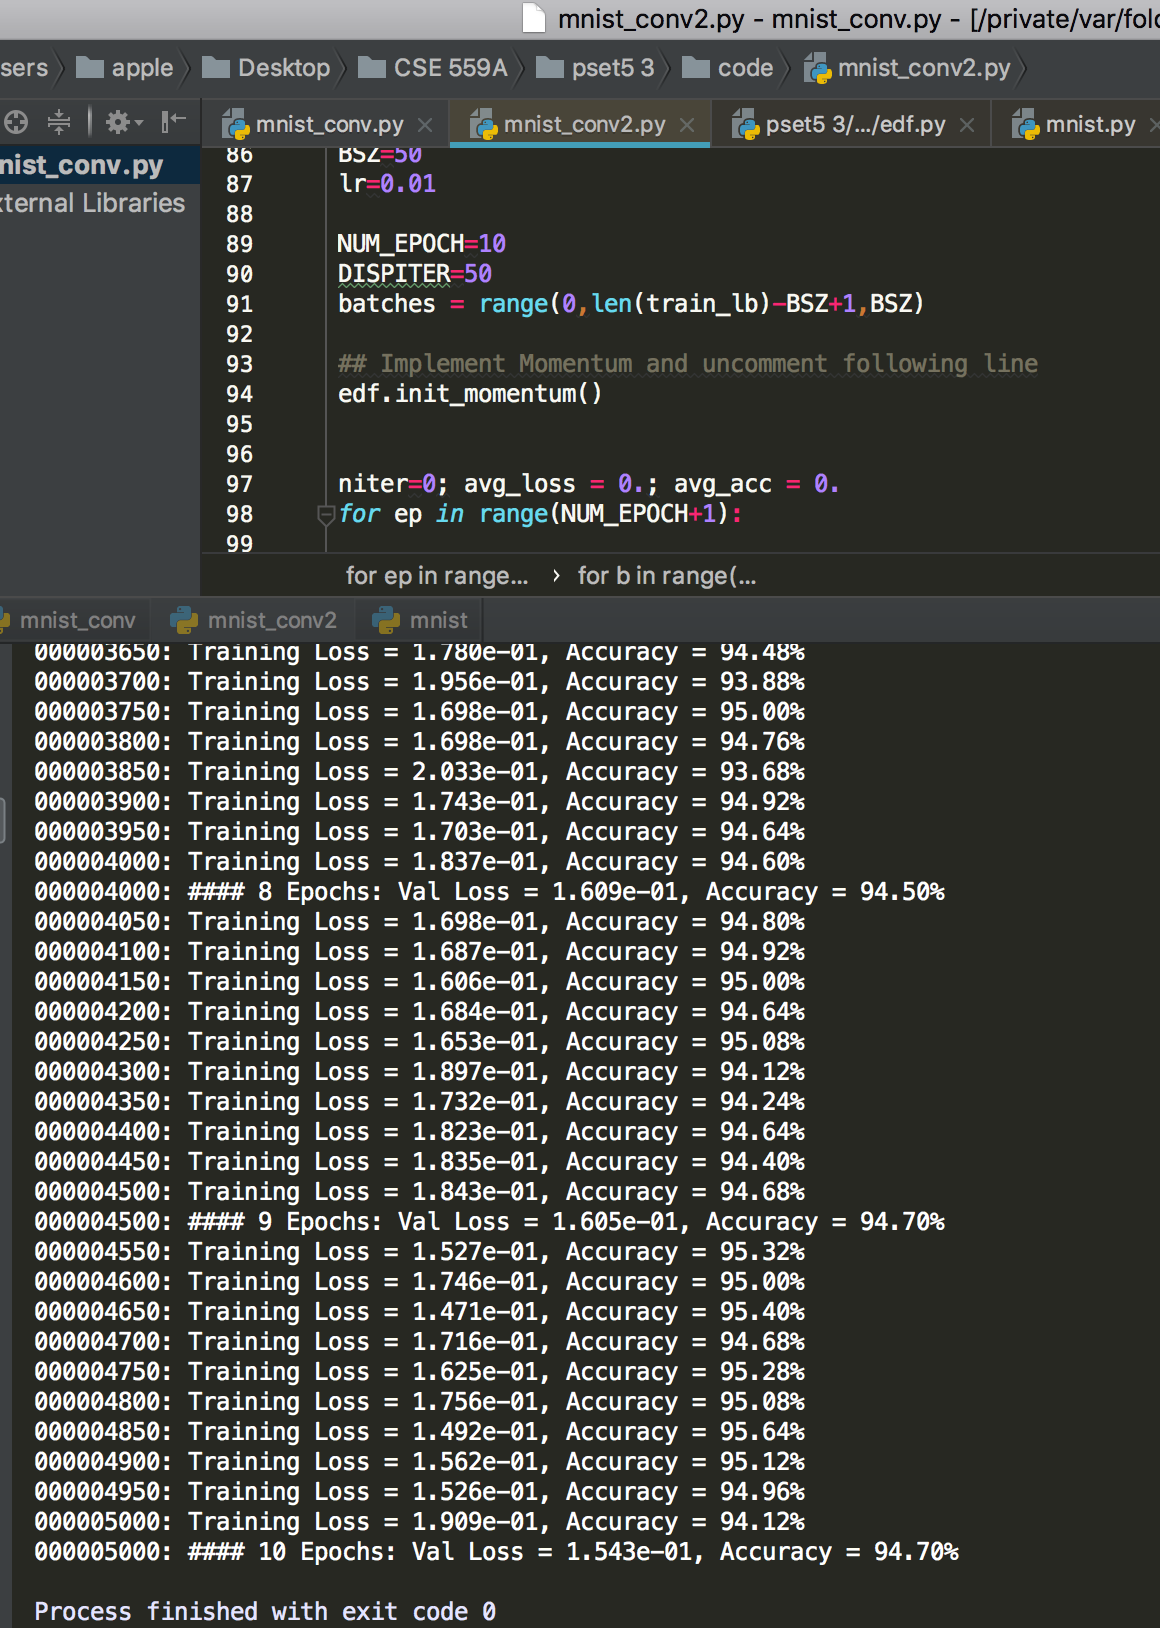
\includegraphics[height=30em]{screenshots/prob3-50-001.png}
	\caption{Processing: Training with momentum under BSZ=50, lr = 0.05}
\end{figure*}
\info

This problem set took approximately 50 hours of effort.

I discussed this problem set with:
\begin{itemize}
\item Sijia Wang
\item Jiarui Xing
\item Ruxin Zhang
\item Chunyuan Li
\end{itemize}

% Note that you might have to escape some special symbols in URLS like \_
I also got hints from the following sources:
\begin{itemize}
\item lecture ppts
\item http://jefkine.com/general/2016/09/05/backpropagation-in-convolutional-neural-networks/
\item http://blog.csdn.net/zhongkejingwang/article/details/44514073
\end{itemize}

\end{document}
